
  \begin{center}
    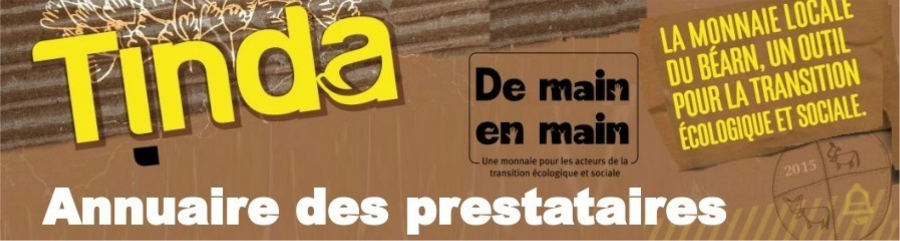
\includegraphics[width=\linewidth]{bandeau_tinda.png}
  \end{center}
\today

    \vspace{.5cm}
    \noindent L’association De Main En Main vous présente l’annuaire des prestataires de la T!nda qui a
vocation à rassembler les acteurs de la transition écologique et sociale en Béarn. Une carte interactive en ligne
    est disponible en plus de cet annuaire (\url{https://carte.demainenmain.org}).
    \vspace{.5cm}

    \noindent La T!nda a pour objectif de soutenir une certaine économie locale, respectueuse des humains et de la nature. la Commission d'agrément de l'association étudie les candidatures des futur·es prestataires en fonction des quatre critères suivants :
    \begin{multicols}{2}
    \begin{itemize}
      \item[\textbf{Territoire}]  Au-delà de l'implantation géographique, nous étudions avec les prestataires la façon dont ils s'engagent dans la vie économique, citoyenne et/ou culturelle de leur territoire, les opportunités d'approvisionnement local, la promotion des circuits-courts et les garanties concernant la qualité des produits et/ou services proposés
	      \vspace{.3cm}
\item[\textbf{Social}] La T!nda, c'est aussi promouvoir les solidarités et la justice sociale. Cela concerne le statut juridique (quel écho avec les valeurs coopératives ?), les valeurs et engagements des prestataires, le souci de proposer un prix juste et les démarches de prévention des risques
    \vspace{.3cm}
\item[\textbf{Environnement}] Nous étudions la prise en compte des enjeux liés à la transition écologique, notamment les leviers pour réduire l'impact sur l'environnement de l'activité
	\vspace{.3cm}
\item[\textbf{Finance}] À quelle banque adhèrent les prestataires ? Ont-ils le souci d'une "valeur ajoutée sociale" ? Nous étudions le mode de gouvernance de la structure et la répartition des bénéfices, nous favorisons leur engagement dans la finance éthique.
    \end{itemize}

  \begin{center}
    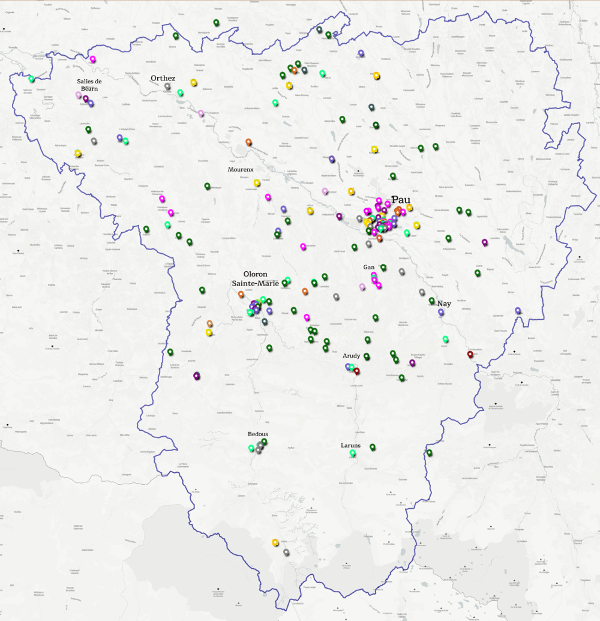
\includegraphics[width=0.9\linewidth]{carte.png}
  \end{center}
\end{multicols}


    \vspace{.2cm}

\noindent Personne n’est parfait, ni même les prestataires de la T!nda ! Mais tous ceux que nous agréons sont déjà engagés d’une façon ou d’une autre dans la transition écologique et sociale qui fera du Béarn un endroit où il fait bon (et encore mieux) vivre ! La T!nda vise à expérimenter un changement lent et fondamental dont chacun·e peut être acteur ou actrice. C'est pourquoi nous faisons le pari, au moment de l'agrément, de relever avec les prestataires un ou plusieurs défi(s) qui permettent de faire vivre en actes la Charte de l'association De Main En Main.
    \vspace{.5cm}


      \textbf{Contact :}
    \begin{itemize}
      \item[] Particuliers : \href{mailto:contact@demainenmain.org}{contact@demainenmain.org}
      \item[] Professionnels : \href{mailto:prestataires@demainenmain.org}{prestataires@demainenmain.org}
      \item[] Mobile : 07 83 29 30 53 
      \item[] Site web : \href{https://www.demainenmain.org}{www.demainenmain.org}
    \end{itemize}

    \vspace{1cm}

  \begin{center}
    {\Large \textbf{Adhérez à De Main En Main et échanger des € contre des T! dans les comptoirs d’échanges !!}}
  \end{center}
